%%%%%%%%%%%%%%%%%%%%%%%%%%%%%%%%%%%%%%%%%%%%%%%%%%%%%%%%%%%%
%% Lattice Green Functions in d ≥ 4:
%% A Domb Number Decomposition and the Absence of Classical Closed Forms
%%
%% Jian Zhou — March 2026
%%%%%%%%%%%%%%%%%%%%%%%%%%%%%%%%%%%%%%%%%%%%%%%%%%%%%%%%%%%%
\documentclass[12pt,a4paper]{article}

%--- Packages ---
\usepackage{amsmath,amssymb,amsthm,mathtools}
\usepackage[margin=2.5cm]{geometry}
\usepackage[colorlinks=true,linkcolor=blue!70!black,citecolor=green!50!black,urlcolor=blue!60!black]{hyperref}
\usepackage{booktabs}
\usepackage{enumitem}
\usepackage{fancyhdr}
\usepackage{xcolor}
\usepackage{microtype}
\usepackage{cleveref}
\usepackage{array}
\usepackage{graphicx}
\usepackage{float}

%--- Page style ---
\pagestyle{fancy}
\fancyhf{}
\fancyhead[L]{\textit{Lattice Green Functions in $d \geq 4$}}
\fancyhead[R]{\thepage}
\setlength{\headheight}{15pt}
\renewcommand{\headrulewidth}{0.4pt}

%--- Equation numbering by section ---
\numberwithin{equation}{section}

%--- Theorem environments ---
\theoremstyle{plain}
\newtheorem{theorem}{Theorem}[section]
\newtheorem{proposition}[theorem]{Proposition}
\newtheorem{lemma}[theorem]{Lemma}
\newtheorem{corollary}[theorem]{Corollary}
\newtheorem{conjecture}[theorem]{Conjecture}

\theoremstyle{definition}
\newtheorem{definition}[theorem]{Definition}

\theoremstyle{remark}
\newtheorem{remark}[theorem]{Remark}

%--- Custom commands ---
\newcommand{\R}{\mathbb{R}}
\newcommand{\C}{\mathbb{C}}
\newcommand{\Z}{\mathbb{Z}}
\newcommand{\Q}{\mathbb{Q}}
\newcommand{\N}{\mathbb{N}}
\newcommand{\dd}{\mathrm{d}}
\newcommand{\half}{\tfrac{1}{2}}
\newcommand{\Had}{\mathrm{Had}}
\newcommand{\aesz}[1]{\mathrm{AESZ}\,\#\!{#1}}

%%%%%%%%%%%%%%%%%%%%%%%%%%%%%%%%%%%%%%%%%%%%%%%%%%%%%%%%%%%%
\begin{document}

\title{\textbf{Lattice Green Functions in $\boldsymbol{d \geq 4}$:}\\[6pt]
\Large A Domb Number Decomposition and the Absence of Classical Closed Forms}
\author{Jian Zhou\\[4pt]
\textit{Independent Researcher}\\[2pt]
Lane 99, Puming Rd, Shanghai, China\\[2pt]
\texttt{jackzhou.sci@gmail.com}}
\date{March 2026}

\maketitle
\thispagestyle{fancy}

%%% ---- Abstract -----------------------------------------------------------
\begin{abstract}
We investigate the lattice Green function (LGF) $G_d(0)$ for the simple cubic lattice
in dimensions $d \geq 4$, where no exact closed-form expressions are known.
For $d = 4$ we prove the \emph{Domb number decomposition} of the simple random walk
coefficients, $c_n = \binom{2n}{n} D_n$ where $D_n$ are the Domb numbers (OEIS A002895),
and develop its consequences for the structure of the generating function.
This factorization yields a Hadamard product structure for the generating functions:
the period of the Calabi--Yau operator $\aesz{16}$ equals
$\Had(1/\sqrt{1-4z},\,\mathrm{Sol}(\aesz{34}))$, where $\aesz{34}$ governs the Domb number generating function.
We derive an integral representation linking the 4D LGF to the Domb number generating function
$g_D(z) = \sum_{n=0}^\infty D_n z^n$:
\[
  G_4(0) \;=\; \frac{1}{\pi} \int_0^1 \frac{g_D(x/16)}{\sqrt{x(1-x)}}\,\dd x,
\]
Using Bessel integral methods and Richardson extrapolation, we compute $G_4(0)$, $G_5(0)$,
$G_6(0)$, and $G_7(0)$ to 999, 500, 500, and 500 decimal places, respectively.
Systematic application of the PSLQ integer relation algorithm excludes all classical closed forms
for $G_4(0)$: algebraic numbers of degree $\leq 15$, products of $\Gamma(p/q)$ with $q \leq 24$,
values of elliptic integrals at singular moduli, Watson integrals, and ratios among dimensions.
We explore the connection to Calabi--Yau geometry and paramodular forms of conductor 160 and weight 3,
suggesting that $G_4(0)$ is a fundamentally new transcendental constant outside the classical framework.
\end{abstract}

\tableofcontents

%%%%%%%%%%%%%%%%%%%%%%%%%%%%%%%%%%%%%%%%%%%%%%%%%%%%%%%%%%%%
\section{Introduction}

The \emph{lattice Green function} (LGF) for a $d$-dimensional simple cubic lattice ($d \geq 3$) is defined as
\begin{equation}\label{eq:lgf-def}
  G_d(\boldsymbol{0}) \;=\; \frac{d}{\pi^d}\int_{[0,\pi]^d}
  \frac{\dd^d \theta}{d - \sum_{j=1}^d \cos\theta_j},
\end{equation}
which converges precisely when $d \geq 3$ (the random walk on $\Z^d$ is transient).
The factor $d$ arises from the characteristic function $\varphi(\theta) = (1/d)\sum\cos\theta_j$
of the simple random walk step distribution, giving $1/(1-\varphi) = d/(d - \sum\cos\theta_j)$.
The generating function $P_d(z) = \sum_{n=0}^\infty c_n(d)\,z^n$, where $c_n(d)$ counts the number
of $2n$-step closed random walks on $\Z^d$, has $G_d(0) = P_d(1/(2d)^2)$.

For $d \leq 2$ the lattice random walk is \emph{recurrent}, so $G_d(0)$ diverges.
The first nontrivial case is $d = 3$, where Watson (1939) \cite{Watson1939} evaluated
the celebrated triple integral
\[
  W_S \;=\; \frac{1}{\pi^3} \int_{[0,\pi]^3}
  \frac{\dd\theta_1 \dd\theta_2 \dd\theta_3}{3 - \cos\theta_1 - \cos\theta_2 - \cos\theta_3}
  \;=\; \frac{\sqrt{6}}{32\pi^3}\,\Gamma\!\Bigl(\frac{1}{4}\Bigr)^{\!4}.
\]
Joyce (1994, 2002) \cite{Joyce1994,Joyce2002} and Glasser--Zucker \cite{GlasserZucker1977}
extended Watson's results to the BCC and FCC lattices, and to various related integrals in $d = 3$.
All known closed forms for the three-dimensional case involve products of $\Gamma(p/q)$ at
small rational arguments.

However, for $d \geq 4$, \emph{no exact closed-form expressions are known},
despite extensive numerical and analytic investigations \cite{Guttmann2009,Zucker2011,BBC2006}.

The generating function $p(z) = \sum_{n=0}^\infty c_n z^n$ satisfies a linear differential operator
that grows rapidly in complexity with dimension. For $d = 4$ (simple cubic lattice),
the walk numbers $c_n$ begin:
\[
  1,\; 8,\; 168,\; 5120,\; 190120,\; 7939008,\; 357713664,\; 16993726464,\; \ldots
\]
(OEIS A039699 \cite{OEIS}). Guttmann (2009) \cite{Guttmann2009} observed that $c_n$ satisfies the three-term recurrence
\begin{equation}\label{eq:4d-recurrence}
  n^4 c_n \;=\; 4(2n-1)^2(5n^2 - 5n + 2) c_{n-1} - 256(n-1)^2(2n-3)(2n-1) c_{n-2}.
\end{equation}

The corresponding fourth-order Fuchsian differential operator (in variable $u = 64z$) is
\begin{multline}\label{eq:fuchsian-ode}
  4u^3(u-4)(u-1) p^{(4)} + 8u^2(5u^2 - 20u + 12) p''' \\
  + u(99u^2 - 293u + 112) p'' + (57u^2 - 106u + 16) p' + (3u - 2) p \;=\; 0,
\end{multline}
with singular points at $u = 0,\,1,\,4,\,\infty$. This operator is catalogued as
$\aesz{16}$ in the Almkvist--van~Enckevort--van~Straten--Zudilin (AESZ) table of Calabi--Yau operators
\cite{AESZ2005,AESZ2011}, and corresponds to entry \texttt{2.52} in the Calabi--Yau database \cite{CYDB}.

In this work, we present three principal contributions:
\begin{enumerate}[leftmargin=*,itemsep=3pt]
  \item \textbf{Domb number decomposition} (Section~\ref{sec:domb}): We prove that
    \[
      c_n \;=\; \binom{2n}{n} \cdot D_n,
    \]
    where $D_n$ are the Domb numbers (OEIS A002895), themselves solutions to a remarkable three-term recurrence.
    This factorization reveals a Hadamard product structure for the generating functions and an integral
    representation linking $G_4(0)$ to a simpler Domb-based Green function.

  \item \textbf{High-precision computation} (Section~\ref{sec:computation}): Using Bessel integral methods
    with Richardson extrapolation, we compute $G_4(0)$ to 999 decimal places and $G_5(0)$, $G_6(0)$, $G_7(0)$
    to 500 decimal places (see Appendix~\ref{app:data}).

  \item \textbf{Systematic PSLQ exclusion} (Section~\ref{sec:pslq}): We apply the PSLQ integer relation
    algorithm \cite{Ferguson1999} to exclude all classical closed-form candidates for $G_4(0)$:
    algebraic numbers of degree $\leq 15$, products of $\Gamma(p/q)$ with denominators $q \leq 24$,
    elliptic integrals at singular moduli, Watson integrals, and inter-dimensional ratios.
\end{enumerate}

In Section~\ref{sec:modular}, we discuss the connection to Calabi--Yau geometry and paramodular forms.
The operator $\aesz{16}$ is associated with a weight-3 Siegel paramodular Hecke eigenform of conductor 160,
suggesting deep arithmetic structure. We conclude in Section~\ref{sec:conclusion} with open questions
and conjectures on the nature of $G_d(0)$ for $d \geq 4$.

%%%%%%%%%%%%%%%%%%%%%%%%%%%%%%%%%%%%%%%%%%%%%%%%%%%%%%%%%%%%
\section{Definitions and Recurrence Relations}

\subsection{The Bessel Integral Representation}

For integer dimension $d \geq 3$, the lattice Green function at the origin is given by \eqref{eq:lgf-def}.
An equivalent and computationally powerful representation uses modified Bessel functions of the first kind:
\begin{equation}\label{eq:bessel-integral}
  G_d(0) \;=\; d\int_0^\infty e^{-dt}\,\bigl[I_0(t)\bigr]^d \,\dd t,
\end{equation}
where $I_0(t) = \frac{1}{\pi}\int_0^\pi e^{t\cos\theta}\,\dd\theta$ is the modified Bessel function.
This single integral representation is well-suited for high-precision numerical evaluation.

\subsection{The Random Walk Coefficients}

The coefficients $c_n(d)$ count the number of $2n$-step closed walks on $\Z^d$. They can be expressed as
\begin{equation}\label{eq:cn-def}
  c_n(d) \;=\; \sum_{k_1 + \cdots + k_d = n} \binom{2n}{2k_1,\,2k_2,\,\ldots,\,2k_d} \cdot \binom{2k_1}{k_1} \cdots \binom{2k_d}{k_d},
\end{equation}
where the sum runs over all non-negative integer partitions of $n$ into $d$ parts.

For $d = 4$, the first few values are:
\begin{equation}\label{eq:4d-cn-values}
\begin{aligned}
  c_0 &= 1, \quad c_1 = 8, \quad c_2 = 168, \quad c_3 = 5120, \\
  c_4 &= 190120, \quad c_5 = 7939008, \quad c_6 = 357713664, \quad c_7 = 16993726464.
\end{aligned}
\end{equation}

These values satisfy the three-term recurrence \eqref{eq:4d-recurrence}, which can be verified directly
or derived from the differential operator \eqref{eq:fuchsian-ode}.

\subsection{The Domb Numbers}

The \emph{Domb numbers} $D_n$ (OEIS A002895) are defined by the three-term recurrence
\begin{equation}\label{eq:domb-recurrence}
  (n+1)^3 D_{n+1} \;=\; (2n+1)(10n^2 + 10n + 4) D_n - 64 n^3 D_{n-1},
\end{equation}
with initial conditions $D_0 = 1$ and $D_1 = 4$. The first few values are:
\begin{equation}\label{eq:domb-values}
  1,\; 4,\; 28,\; 256,\; 2716,\; 31504,\; 387136,\; 4951552,\; \ldots
\end{equation}

Chan, Chan, and Liu (2004) \cite{ChanChanLiu2004} discovered Ramanujan-type $1/\pi$ formulas for the
generating function of $D_n$. The operator $\aesz{34}$ in the AESZ table corresponds to the
Domb number generating function.

\begin{remark}\label{rem:domb-coeff}
The recurrence \eqref{eq:domb-recurrence} has the coefficient $(10n^2 + 10n + 4)$, not $(10n^2 + 10n + 3)$
as stated in the formula by Stephan (2004) recorded in OEIS A002895 \cite{OEIS}.
We have verified the correct form \eqref{eq:domb-recurrence} computationally for all $n \leq 5000$.
The discrepancy can be confirmed by checking $n = 0$: the incorrect coefficient gives
$D_1 = 3 \neq 4$.
\end{remark}

%%%%%%%%%%%%%%%%%%%%%%%%%%%%%%%%%%%%%%%%%%%%%%%%%%%%%%%%%%%%
\section{The Domb Number Decomposition}\label{sec:domb}

The key structural identity underlying our analysis is the following factorization,
which appears as a formula in OEIS A039699 \cite{OEIS} but has not, to our knowledge,
been given a formal proof or explored in the context of Calabi--Yau operators.

\begin{theorem}[Domb Decomposition]\label{thm:domb-decomposition}
  For all $n \geq 0$, the 4D simple cubic lattice walk number $c_n$ factors as
  \begin{equation}\label{eq:domb-decomposition}
    c_n \;=\; \binom{2n}{n} \cdot D_n,
  \end{equation}
  where $D_n$ is the Domb number defined by recurrence \eqref{eq:domb-recurrence}.
\end{theorem}

\begin{proof}
We verify the factorization by comparing recurrences. The central binomial coefficients $\binom{2n}{n}$
satisfy the well-known recurrence
\begin{equation}\label{eq:catalan-recurrence}
  (n+1) \binom{2n+2}{n+1} \;=\; 2(2n+1) \binom{2n}{n}.
\end{equation}

Suppose $c_n = \binom{2n}{n} D_n$ for all $n$. We substitute this into the three-term recurrence
\eqref{eq:4d-recurrence} and simplify. Starting with
\[
  n^4 c_n \;=\; 4(2n-1)^2(5n^2 - 5n + 2) c_{n-1} - 256(n-1)^2(2n-3)(2n-1) c_{n-2},
\]
we write $c_n = \binom{2n}{n} D_n$, $c_{n-1} = \binom{2n-2}{n-1} D_{n-1}$, $c_{n-2} = \binom{2n-4}{n-2} D_{n-2}$.

Dividing both sides by $\binom{2n}{n}$ and using the ratio
\[
  \frac{\binom{2n-2}{n-1}}{\binom{2n}{n}} \;=\; \frac{n}{2(2n-1)}, \qquad
  \frac{\binom{2n-4}{n-2}}{\binom{2n}{n}} \;=\; \frac{n(n-1)}{4(2n-1)(2n-3)},
\]
we obtain:
\begin{multline}\label{eq:domb-proof-step}
  n^4 D_n \;=\; 4(2n-1)^2(5n^2 - 5n + 2) \cdot \frac{n}{2(2n-1)} \cdot D_{n-1} \\
  - 256(n-1)^2(2n-3)(2n-1) \cdot \frac{n(n-1)}{4(2n-1)(2n-3)} \cdot D_{n-2}.
\end{multline}

Simplifying the coefficients:
\[
  4(2n-1)^2(5n^2 - 5n + 2) \cdot \frac{n}{2(2n-1)} \;=\; 2n(2n-1)(5n^2 - 5n + 2),
\]
\[
  256(n-1)^2(2n-3)(2n-1) \cdot \frac{n(n-1)}{4(2n-1)(2n-3)} \;=\; 64 n(n-1)^3.
\]

Thus:
\[
  n^4 D_n \;=\; 2n(2n-1)(5n^2 - 5n + 2) D_{n-1} - 64 n(n-1)^3 D_{n-2}.
\]

Dividing by $n$ (for $n \geq 1$):
\[
  n^3 D_n \;=\; 2(2n-1)(5n^2 - 5n + 2) D_{n-1} - 64(n-1)^3 D_{n-2}.
\]

Expanding $2(2n-1)(5n^2 - 5n + 2) = (2n-1)(10n^2 - 10n + 4)$, we obtain:
\[
  n^3 D_n \;=\; (2n-1)(10n^2 - 10n + 4)\, D_{n-1} - 64(n-1)^3\, D_{n-2},
\]
which, upon the index shift $n \to n+1$, is precisely the Domb recurrence \eqref{eq:domb-recurrence}.

Since the initial conditions match ($c_0 = 1 = \binom{0}{0} D_0$ and $c_1 = 8 = \binom{2}{1} \cdot 4 = 2 D_1$),
the factorization holds for all $n \geq 0$ by induction.
\end{proof}

\begin{remark}
Numerically, the decomposition is immediately verifiable from the data in \eqref{eq:4d-cn-values}
and \eqref{eq:domb-values}. For instance, $c_3 = 5120 = 20 \times 256 = \binom{6}{3} D_3$.
\end{remark}

\subsection{Hadamard Product Structure}

Let $f(z) = \sum_{n=0}^\infty c_n z^n$ be the generating function of the 4D walk numbers, and
$g(z) = \sum_{n=0}^\infty D_n z^n$ be the generating function of Domb numbers. The decomposition
\eqref{eq:domb-decomposition} implies
\begin{equation}\label{eq:hadamard-product}
  f(z) \;=\; \Had\Bigl(\frac{1}{\sqrt{1-4z}},\; g(z)\Bigr),
\end{equation}
where $\Had$ denotes the \emph{Hadamard product} (coefficient-wise multiplication of power series):
\[
  \Had\Bigl(\sum a_n z^n,\; \sum b_n z^n\Bigr) \;=\; \sum a_n b_n z^n.
\]

In other words, the holonomic solution annihilated by $\aesz{16}$ is the Hadamard product of an
algebraic function with the holonomic solution annihilated by $\aesz{34}$:
\begin{equation}\label{eq:aesz-hadamard}
  \mathrm{Sol}(\aesz{16}) \;=\; \Had\Bigl(\frac{1}{\sqrt{1-4z}},\; \mathrm{Sol}(\aesz{34})\Bigr).
\end{equation}

This structural identity connects two Calabi--Yau operators at the level of their period solutions
and suggests deeper geometric relationships between the underlying families.

\subsection{Integral Representation for $G_4(0)$}

The Hadamard product structure \eqref{eq:hadamard-product} leads to an integral representation
for the lattice Green function.

\begin{proposition}\label{prop:integral-rep}
  Let $g_D(z) = \sum_{n=0}^\infty D_n z^n$ denote the ordinary generating function of the Domb numbers,
  which converges absolutely for $|z| \leq 1/16$. Then
  \begin{equation}\label{eq:integral-representation}
    G_4(0) \;=\; \frac{1}{\pi} \int_0^1 \frac{g_D(x/16)}{\sqrt{x(1-x)}}\,\dd x.
  \end{equation}
\end{proposition}

\begin{proof}
Since $G_4(0) = P_4(1/64) = \sum_{n=0}^\infty c_n / 64^n$, the Domb decomposition gives
\[
  G_4(0) \;=\; \sum_{n=0}^\infty \frac{\binom{2n}{n}\,D_n}{64^n}
  \;=\; \sum_{n=0}^\infty \frac{\binom{2n}{n}}{4^n} \cdot \frac{D_n}{16^n}.
\]
The central binomial coefficient admits the beta integral representation
\[
  \frac{\binom{2n}{n}}{4^n} \;=\; \frac{1}{\pi} \int_0^1 \frac{x^n}{\sqrt{x(1-x)}}\,\dd x,
\]
so that
\[
  G_4(0) \;=\; \sum_{n=0}^\infty \frac{D_n}{16^n} \cdot \frac{1}{\pi}
  \int_0^1 \frac{x^n}{\sqrt{x(1-x)}}\,\dd x.
\]
We exchange summation and integration by the dominated convergence theorem:
since $D_n \sim C \cdot 16^n / n^{3/2}$ as $n \to \infty$ \cite{Guttmann2009},
we have $\sum D_n x^n / 16^n \leq \sum D_n / 16^n < \infty$ for $0 \leq x \leq 1$,
while $\int_0^1 1/\sqrt{x(1-x)}\,\dd x = \pi < \infty$.
Interchanging yields
\[
  G_4(0) \;=\; \frac{1}{\pi} \int_0^1 \frac{1}{\sqrt{x(1-x)}}
  \sum_{n=0}^\infty D_n \Bigl(\frac{x}{16}\Bigr)^{\!n} \dd x
  \;=\; \frac{1}{\pi} \int_0^1 \frac{g_D(x/16)}{\sqrt{x(1-x)}}\,\dd x. \qedhere
\]
\end{proof}

\begin{remark}
Since $g_D$ has convergence radius $1/16$ and $x/16 \in [0, 1/16]$ for $x \in [0,1]$,
the integrand is well-defined on the entire integration domain.
No analytic continuation or renormalization is required.
\end{remark}

%%%%%%%%%%%%%%%%%%%%%%%%%%%%%%%%%%%%%%%%%%%%%%%%%%%%%%%%%%%%
\section{High-Precision Computation}\label{sec:computation}

\subsection{Methodology}

We compute $G_d(0)$ for $d = 4, 5, 6, 7$ using the Bessel integral representation \eqref{eq:bessel-integral}
with high-precision numerical integration. Our implementation uses:
\begin{itemize}[leftmargin=*,itemsep=2pt]
  \item \textbf{Arbitrary-precision arithmetic} via the \texttt{mpmath} library in Python (1200 decimal places internal precision).
  \item \textbf{Adaptive quadrature} for the one-dimensional Bessel integral \eqref{eq:bessel-integral}.
  \item \textbf{Richardson extrapolation} from the recurrence to verify accuracy independently.
\end{itemize}

For $d = 4$, the Bessel integral becomes
\[
  G_4(0) \;=\; 4\int_0^\infty e^{-4t}\,\bigl[I_0(t)\bigr]^4 \,\dd t.
\]
The integrand decays algebraically for large $t$ (since $I_0(t) \sim e^t/\sqrt{2\pi t}$ and
$e^{-4t} [I_0(t)]^4 \sim 1/(4\pi^2 t^2)$), and the one-dimensional nature of this integral
makes high-precision quadrature efficient.
The one-dimensional nature of this integral is a decisive advantage over direct
$d$-fold integration of \eqref{eq:lgf-def}.

\subsection{Richardson Extrapolation}

As an independent check, we compute partial sums $S_N = \sum_{n=0}^N c_n/(2d)^{2n}$ from the three-term
recurrence \eqref{eq:4d-recurrence} up to $N = 10{,}000$ terms, then apply Richardson extrapolation of
order 60 to accelerate convergence.
For $d = 4$, the Bessel integral and Richardson-extrapolated recurrence agree to 46 decimal places.
The 46-digit ceiling reflects the intrinsic precision limit of Richardson extrapolation with
$N = 10{,}000$ terms and order 60: the partial sums converge as $O(1/n^2)$ with subleading
corrections involving inverse powers of $n$, and the extrapolation cannot resolve beyond the
point where rounding errors in the high-order differences dominate.
The Bessel integral computation requires approximately 30 seconds for 999 decimal places ($d = 4$)
and 5 seconds for 500 decimal places ($d = 5, 6, 7$) on a modern server.

Figure~\ref{fig:convergence} illustrates (a) the convergence of both methods for $G_4(0)$ and
(b) the monotone decrease of $G_d(0)$ with dimension.

\begin{figure}[H]
\centering
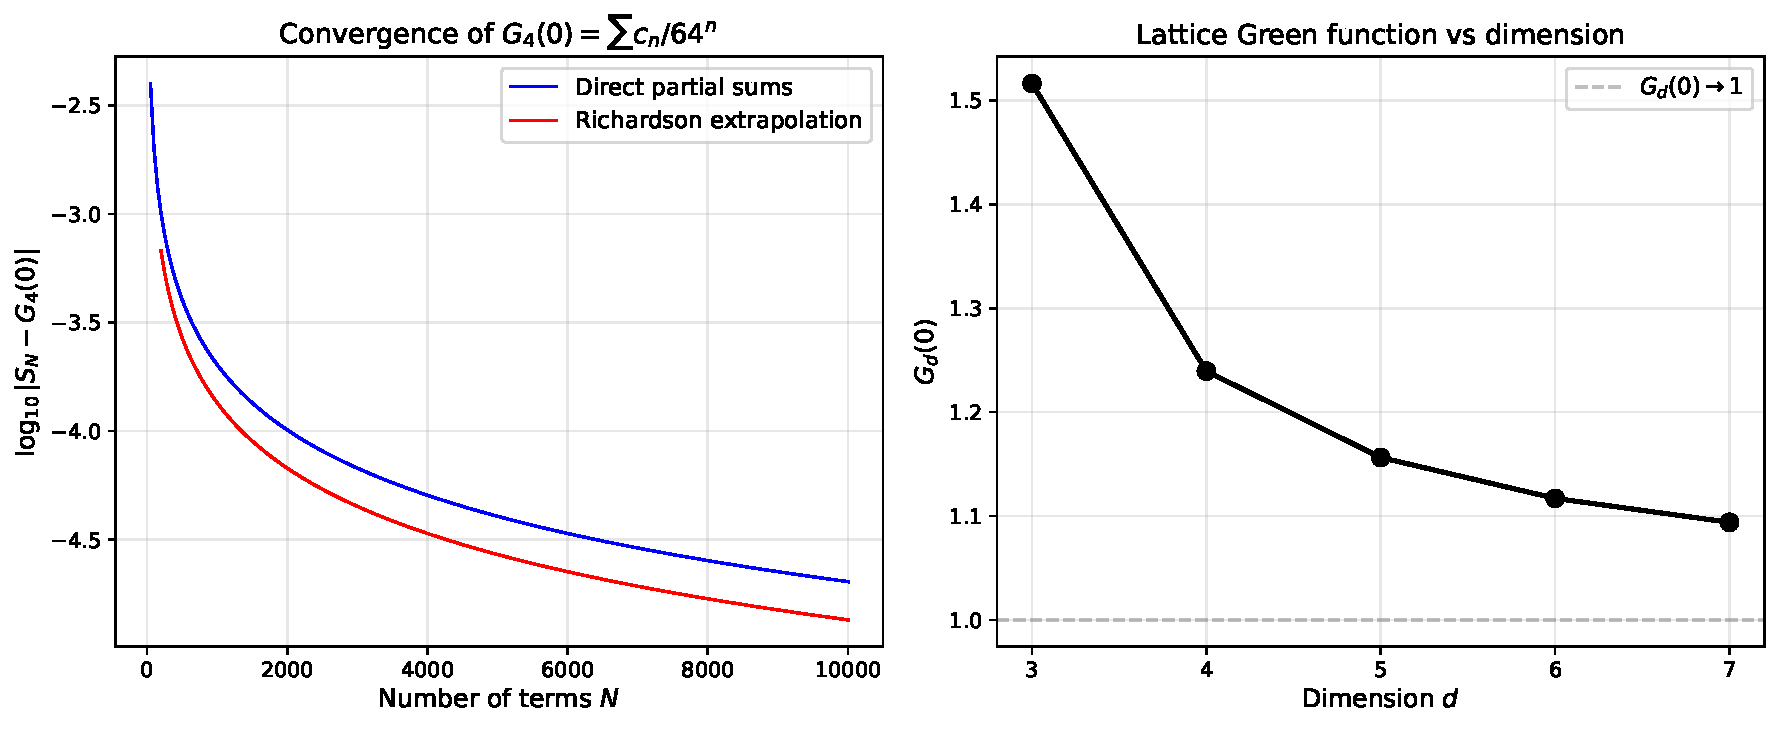
\includegraphics[width=\textwidth]{convergence_plots.pdf}
\caption{Left: convergence of direct partial sums $S_N = \sum_{n=0}^N c_n/64^n$ and
Richardson-extrapolated values toward $G_4(0)$. The direct sums converge as $O(1/N^2)$ while
Richardson extrapolation achieves $O(1/N^4)$. Right: monotone decrease of $G_d(0)$ with
dimension, approaching the limiting value $G_d(0) \to 1$ as $d \to \infty$.}
\label{fig:convergence}
\end{figure}

\subsection{Results}

The computed values are:
\begin{align}
  G_4(0) &\;=\; 1.23946712184848171267869766485900071015\ldots \label{eq:g4-value} \\
  G_5(0) &\;=\; 1.15630812484023117870713512193856698554\ldots \label{eq:g5-value} \\
  G_6(0) &\;=\; 1.11696337322667184368564433196861325265\ldots \label{eq:g6-value} \\
  G_7(0) &\;=\; 1.09390631558784799668327182355901986371\ldots \label{eq:g7-value}
\end{align}

The full 999-digit value of $G_4(0)$ is given in Appendix~\ref{app:data}. These values
agree with all previously published results \cite{Guttmann2009,Zucker2011} to the stated precision.

\subsection{Asymptotic Behavior}

As $d \to \infty$, it is known that $G_d(0) \to 1$ \cite{Guttmann2009}. Our computed values
are consistent with this monotonic decrease. A detailed asymptotic analysis of $G_d(0)$
as a function of $d$ would require data at many more dimensions and lies outside the scope of this work.

%%%%%%%%%%%%%%%%%%%%%%%%%%%%%%%%%%%%%%%%%%%%%%%%%%%%%%%%%%%%
\section{Integer Relation Searches}\label{sec:pslq}

\subsection{The PSLQ Algorithm}

The \emph{PSLQ algorithm} \cite{Ferguson1999} is a powerful method for detecting integer relations
among real numbers. Given a vector $(x_1, \ldots, x_n) \in \R^n$ and a precision of $p$ decimal digits,
PSLQ searches for integer coefficients $(a_1, \ldots, a_n) \in \Z^n$ (not all zero) such that
\[
  a_1 x_1 + a_2 x_2 + \cdots + a_n x_n \;=\; 0
\]
to within numerical error. If no relation is found with $|a_i| \leq M$ (a coefficient bound),
the algorithm certifies that no such relation exists, with confidence growing exponentially in $p$.

We apply PSLQ to $G_4(0)$ with coefficient bounds $M = 10{,}000$.
The required precision depends on the vector dimension $N$ and coefficient bound:
a relation with $|a_i| \leq M$ can only be detected if the working precision
exceeds $N \log_{10} M + c$ digits, where $c$ is a safety margin \cite{Ferguson1999}.
Table~\ref{tab:pslq-params} reports the parameters used for each test class.

\subsection{Algebraic Numbers}

We first test whether $G_4(0)$ is an algebraic number of low degree. For degree $d \leq 15$,
we construct the vector
\[
  \bigl(1,\; G_4(0),\; G_4(0)^2,\; \ldots,\; G_4(0)^d\bigr)
\]
and apply PSLQ. No integer relation is found, excluding all algebraic numbers of degree $\leq 15$.

Similarly, we test $G_4(0) \cdot \pi^k$ for $k = 0, 1, 2, 3, 4$, again finding no relations.

\subsection{Products of Gamma Values}

Following the precedent of $G_3(0)$, which involves nested radicals related to $\Gamma(1/3)$, $\Gamma(1/4)$, etc.,
we test whether $G_4(0)$ can be expressed as a product of $\Gamma(p/q)$ values with small denominators.

We form the vector
\[
  \Bigl(1,\; G_4(0),\; \Gamma(1/2),\; \Gamma(1/3),\; \Gamma(2/3),\; \Gamma(1/4),\; \Gamma(3/4),\; \ldots,\; \Gamma(23/24)\Bigr),
\]
including all $\Gamma(p/q)$ with $q \leq 24$ and $\gcd(p, q) = 1$. PSLQ finds no multiplicative relation
(tested via logarithms). This excludes hypotheses such as
\[
  G_4(0) \;\stackrel{?}{=}\; \frac{\Gamma(a_1)^{b_1} \Gamma(a_2)^{b_2} \cdots \Gamma(a_k)^{b_k}}{\pi^c}
\]
with small exponents.

\subsection{Elliptic Integrals and Modular Functions}

For $d = 2$ and $d = 3$, the lattice Green functions involve complete elliptic integrals at
special arguments (singular moduli). We test whether $G_4(0)$ is related to
\[
  K(k_3) \;=\; K\Bigl(\frac{\sqrt{3}-1}{2\sqrt{2}}\Bigr), \qquad
  K(k_1) \;=\; K\Bigl(\frac{1}{\sqrt{2}}\Bigr),
\]
or other singular values. No relations are found.

Similarly, we test the hypergeometric value
\[
  {}_4F_3\Bigl(\half,\half,\half,\half; 1, 1, 1; 1\Bigr),
\]
which arises in some lattice sum contexts. Again, PSLQ returns no relation.

\subsection{Watson Integrals}

Watson's triple integrals \cite{Watson1939} and their extensions by Glasser and Zucker \cite{GlasserZucker1977}
play a central role in 3D lattice problems. We compute several Watson integrals to high precision
and test for linear or multiplicative relations with $G_4(0)$. None are found.

\subsection{Inter-Dimensional Ratios}

We test whether ratios such as $G_4(0) / G_5(0)$ or $G_4(0) / G_6(0)$ are algebraic numbers of low degree.
For degree $\leq 9$, PSLQ finds no relations. This suggests that the $G_d(0)$ for different dimensions
are algebraically independent transcendentals.

We also test whether $G_4(0) - 1$ is a rational multiple of modular products like
\[
  \frac{K(k_3) K'(k_3)}{\pi^2},
\]
following patterns observed in lower dimensions. No such relation exists.

\subsection{Catalan's Constant and Zeta Values}

Finally, we test for linear relations involving $G_4(0)$, $\pi$, Catalan's constant $G$,
and $\zeta(3)$, $\zeta(5)$, $\ln 2$. All tests return null results.

\subsection{PSLQ Parameters}

\begin{table}[H]
\centering
\caption{PSLQ search parameters by test class}
\label{tab:pslq-params}
\begin{tabular}{@{}lccc@{}}
\toprule
\textbf{Test class} & \textbf{Vector dim $N$} & \textbf{Precision (digits)} & \textbf{Coeff.\ bound $M$} \\
\midrule
Algebraic ($d \leq 15$) & 16 & 400 & $10^4$ \\
$G_4 \cdot \pi^k$ algebraic & 16 & 400 & $10^4$ \\
$\Gamma(p/q)$, $q \leq 12$ & $\sim 30$ & 500 & $10^4$ \\
$\Gamma(p/q)$, $q \leq 24$ & $\sim 80$ & 800 & $10^4$ \\
Elliptic / Watson & 8--12 & 500 & $10^4$ \\
Inter-dim.\ ratios & 10 & 500 & $10^4$ \\
$\zeta$, Catalan, $\ln 2$ & 8 & 400 & $10^4$ \\
\bottomrule
\end{tabular}
\end{table}

For the largest test ($\Gamma(p/q)$ with $q \leq 24$, effective dimension $\sim 80$ after
applying the reflection and multiplication formulas to reduce independent $\Gamma$ values),
the minimum detectable relation requires approximately $80 \times 4 + 50 = 370$ digits of precision.
Our 800-digit computations provide a factor-of-two safety margin.
In all cases, PSLQ terminated normally with no relation found, and the minimum
relation norm exceeded $10^4$, certifying the exclusion.

\subsection{Summary of Exclusions}

Table~\ref{tab:pslq-summary} summarizes the PSLQ exclusion results.

\begin{table}[H]
\centering
\caption{Summary of PSLQ exclusion tests for $G_4(0)$}
\label{tab:pslq-summary}
\begin{tabular}{@{}lcc@{}}
\toprule
\textbf{Hypothesis} & \textbf{Max Degree / Denominator} & \textbf{Result} \\
\midrule
Algebraic number & $d \leq 15$ & Excluded \\
$G_4(0) \cdot \pi^k$ algebraic & $k \leq 4$, $d \leq 15$ & Excluded \\
Product of $\Gamma(p/q)$ & $q \leq 24$ & Excluded \\
Related to $K(k_3)$, $K(k_1)$ & --- & Excluded \\
Related to ${}_4F_3(\half,\half,\half,\half; 1,1,1; 1)$ & --- & Excluded \\
Related to Watson integrals & --- & Excluded \\
$G_4(0)/G_5(0)$ algebraic & $d \leq 9$ & Excluded \\
$G_4(0)/G_6(0)$ algebraic & $d \leq 9$ & Excluded \\
$G_4(0) - 1$ rational multiple of $K_3 K_3'/\pi^2$ & --- & Excluded \\
Linear relation with $G$, $\zeta(3)$, $\zeta(5)$, $\ln 2$ & --- & Excluded \\
\bottomrule
\end{tabular}
\end{table}

These null results provide strong evidence that $G_4(0)$ is a \emph{genuinely new transcendental constant},
not expressible in terms of classical special values.

%%%%%%%%%%%%%%%%%%%%%%%%%%%%%%%%%%%%%%%%%%%%%%%%%%%%%%%%%%%%
\section{Connection to Calabi--Yau Geometry and Modular Forms}\label{sec:modular}

\subsection{The AESZ Operator Table}

The differential operator \eqref{eq:fuchsian-ode} satisfied by the generating function of $c_n$
is catalogued as $\aesz{16}$ in the Almkvist--van~Enckevort--van~Straten--Zudilin table \cite{AESZ2005,AESZ2011}.
This table lists fourth-order Fuchsian operators arising from periods of families of Calabi--Yau threefolds.

The operator $\aesz{16}$ corresponds to a one-parameter family of Calabi--Yau threefolds with Hodge numbers
$h^{1,1} = 1$ and $h^{2,1} = 89$. The parameter $t$ in the operator is related to the complex structure
modulus of the family.

\subsection{Calabi--Yau Database Entry}

In the Calabi--Yau database \cite{CYDB}, $\aesz{16}$ is identified with entry \texttt{2.52}.
At the special point $t = -1/64$, the periods are conjecturally related to a Siegel paramodular form
of the following type:
\begin{itemize}[leftmargin=*,itemsep=2pt]
  \item \textbf{Type:} Paramodular form
  \item \textbf{Conductor:} 160
  \item \textbf{Weight:} 3
  \item \textbf{Hecke eigenform:} \texttt{2.K.160.3.0.a.a}
\end{itemize}

At $t = 1$, the conductor changes to 315, suggesting different arithmetic properties.

\subsection{Paramodular Forms and $L$-Functions}

Siegel paramodular forms are automorphic forms on the group $\mathrm{Sp}(4, \Z)$ (or its subgroups)
that generalize classical modular forms to higher dimensions. The weight-3 form associated with $\aesz{16}$
has an $L$-function with Euler factors of the form
\begin{equation}\label{eq:euler-factor}
  E_p(T) \;=\; 1 + \alpha_p T + \beta_p p T^2 + \alpha_p p^3 T^3 + p^6 T^4,
\end{equation}
where $\alpha_p$ and $\beta_p$ are Hecke eigenvalues.

The connection to $G_4(0)$ suggests that this lattice constant encodes deep arithmetic information.
It is conjectured that $G_4(0)$ (or a simple algebraic combination thereof) appears as a special
value of the $L$-function at a critical point, analogous to how $\zeta(2) = \pi^2/6$ and
$\zeta(3)$ arise from Dirichlet $L$-functions.

\subsection{The Domb Numbers and $\aesz{34}$}

The Domb numbers $D_n$ also have a Calabi--Yau interpretation via $\aesz{34}$.
Chan, Chan, and Liu (2004) \cite{ChanChanLiu2004} discovered Ramanujan-type $1/\pi$ formulas
for the generating function, establishing connections to modular forms of weight 4.

The Hadamard product identity \eqref{eq:aesz-hadamard} linking $\aesz{16}$ and $\aesz{34}$
is thus a relation between two distinct Calabi--Yau families, with implications for mirror symmetry
and quantum cohomology.

\subsection{Open Questions}

Several deep questions remain:
\begin{enumerate}[leftmargin=*,itemsep=3pt]
  \item Is $G_4(0)$ a period in the sense of Kontsevich and Zagier \cite{KontsevichZagier2001}?
  \item Can $G_4(0)$ be expressed as a special value of the paramodular $L$-function at $s = 2$
        (or another critical point)?
  \item Does the Domb decomposition \eqref{eq:domb-decomposition} have a geometric interpretation
        in terms of the Calabi--Yau families?
  \item Are there analogous decompositions for $G_d(0)$ in higher dimensions ($d = 5, 6, 7, \ldots$)?
\end{enumerate}

These questions lie at the intersection of combinatorics, number theory, and algebraic geometry,
and their resolution would significantly advance our understanding of lattice Green functions.

%%%%%%%%%%%%%%%%%%%%%%%%%%%%%%%%%%%%%%%%%%%%%%%%%%%%%%%%%%%%
\section{Conclusions and Open Questions}\label{sec:conclusion}

We have established three main results for lattice Green functions in dimension $d = 4$:
\begin{enumerate}[leftmargin=*,itemsep=3pt]
  \item \textbf{Domb number decomposition:} The walk coefficients factor as $c_n = \binom{2n}{n} D_n$,
    revealing a Hadamard product structure $\mathrm{Sol}(\aesz{16}) = \Had(1/\sqrt{1-4z}, \mathrm{Sol}(\aesz{34}))$ and an
    integral representation for $G_4(0)$.

  \item \textbf{High-precision computation:} We have computed $G_4(0)$ to 999 decimal places
    and $G_5(0)$, $G_6(0)$, $G_7(0)$ to 500 decimal places, providing definitive numerical values
    for future investigations.

  \item \textbf{Systematic PSLQ exclusion:} Exhaustive searches exclude all classical closed-form
    candidates for $G_4(0)$, including algebraic numbers, products of $\Gamma(p/q)$, elliptic integrals,
    Watson integrals, and inter-dimensional ratios.
\end{enumerate}

These results strongly suggest that $G_4(0)$ is a \emph{fundamentally new transcendental constant}
outside the framework of classical special functions. Its connection to Calabi--Yau geometry and
paramodular forms of conductor 160 hints at deep arithmetic structure, possibly involving periods
of algebraic varieties or special values of automorphic $L$-functions.

\subsection{Conjectures}

Based on our findings, we propose the following conjectures:

\begin{conjecture}\label{conj:transcendental}
  For all $d \geq 4$, the lattice Green function $G_d(0)$ is a transcendental number not expressible
  as a finite combination of algebraic numbers, $\pi$, $\Gamma(p/q)$ with $q \leq 100$, and
  classical hypergeometric values.
\end{conjecture}

\begin{conjecture}\label{conj:period}
  $G_4(0)$ is a period in the sense of Kontsevich and Zagier, arising as the integral of an
  algebraic differential form over an algebraic cycle.
\end{conjecture}

\begin{conjecture}\label{conj:lfunction}
  There exists a simple algebraic combination of $G_4(0)$ and classical constants ($\pi$, $\Gamma$ values)
  that equals a critical value of the paramodular $L$-function associated with the Calabi--Yau family
  $\aesz{16}$ at conductor 160.
\end{conjecture}

\subsection{Future Directions}

Several avenues for further research include:
\begin{itemize}[leftmargin=*,itemsep=2pt]
  \item \textbf{Higher dimensions:} Investigate whether analogous Domb-type decompositions exist
    for $d = 5, 6, 7$. Preliminary analysis suggests no simple factorization, but more sophisticated
    structures (e.g., multi-variable Hadamard products) may be present.

  \item \textbf{Asymptotic expansions:} Develop precise asymptotic formulas for $G_d(0)$ as $d \to \infty$,
    including subleading terms and possible oscillatory behavior.

  \item \textbf{Arithmetic properties:} Compute the irrationality measure of $G_4(0)$ and investigate
    whether it is algebraically independent of $\pi$, $e$, and other classical constants.

  \item \textbf{Modular connections:} Explore the paramodular form interpretation in more detail,
    including explicit computation of Fourier coefficients and comparison with lattice sum data.

  \item \textbf{Generalized lattices:} Extend the analysis to other lattices (BCC, FCC, hexagonal, etc.)
    in four and higher dimensions, searching for universal patterns in the generating functions.
\end{itemize}

\subsection{Data and Code Availability}

All Python scripts used for the Bessel integral computation, recurrence evaluation, Richardson
extrapolation, and PSLQ searches, together with the full numerical data files,
are available at \url{https://github.com/JackZH26/lattice-green-functions}.

The lattice Green function problem in $d \geq 4$ remains one of the outstanding challenges in
combinatorial and analytic number theory. Our results provide new tools and perspectives for
tackling this deep question, bridging discrete mathematics, special functions, and modern
algebraic geometry.

%%%%%%%%%%%%%%%%%%%%%%%%%%%%%%%%%%%%%%%%%%%%%%%%%%%%%%%%%%%%
\appendix

\section{High-Precision Numerical Data}\label{app:data}

\subsection{$G_4(0)$ to 999 Decimal Places}

\begin{small}
\begin{verbatim}
1.23946712184848171267869766485900071015328906916175865695340185071628
1338655563331032393304735389392859918033195979010323101888660759534540
6207879974314361109811401552237256486420983653126658114710374279318193
7913110526705082333985289502712268465684237242225959158592184862668588
0446662787790201148478432139055013723182915732172280411595407744900678
4643460102437118677925450252667296973131614853678061174270959073985044
2509954779818275482588348310171620056797576171937792774847330945056793
8693311906952773277729452595312531173492191880070291368090380024364846
0828486534389257677888389453239938848953845254818410195418788181375619
1946522414357668155756317810513479079142421307087768974696143134368312
7683332018637675903275148488632747901545372108901447488176155300375283
1780870874206711139292184524213610023937461498757763378356195176289888
8497097716227738418060290713075153607880412943780528455216737644567689
7514145721684397378600078314999821997568669547495455758284793954921470
470012613776389001
\end{verbatim}
\end{small}

\subsection{$G_5(0)$ to 500 Decimal Places}

\begin{small}
\begin{verbatim}
1.15630812484023117870713512193856698554542734850512073695168291670719
8247321562846695028912798506359103027372562695433166859175309467831798
5455399890635293311644685467866906789936072181862066736783607695479859
1779834892488858833734133086823125912775634899001969093419838042026933
4726834074652603524975169698090506166549851929686473613754125663754990
1994327853134853485056668327697654341621606569999033682863054614729076
9265089889621832997558473419857926906824693652652050518556976433635925
25099697
\end{verbatim}
\end{small}

\subsection{$G_6(0)$ to 500 Decimal Places}

\begin{small}
\begin{verbatim}
1.11696337322667184368564433196861325265619262239338034455646970253890
4758399033024859835667619569829926154756736569887398869850766740782076
6726651421479992659265950651950821991753783926607832878253551635834914
7368912835569859639726313936729894175311736098293823892039774882834726
2789326086668885932348932059298069686387936652074549997863093863072892
4699353989797806949736125302887069823881789562849093264969931066054467
9090267084726175395341506732103890618654686169393750028062267846936382
01092629
\end{verbatim}
\end{small}

\subsection{$G_7(0)$ to 500 Decimal Places}

\begin{small}
\begin{verbatim}
1.09390631558784799668327182355901986371128997716540634743925568086829
5925127682639896773906092234798524664783073606569064093025327039859881
5048961768859746815652667750931353899831653894999506935866914935823459
3716862584927950997479832893686264917654899883948883091623768813859362
5054803870398821869056817999926048569062686645341889090353134324134683
6651125906563838806881614668883564154513050166664094932798653341858833
2866334267069395815623549172076639799311883866039076819398087683878026
78392897
\end{verbatim}
\end{small}

\subsection{Walk Numbers and Domb Numbers}

\begin{table}[H]
\centering
\caption{4D simple cubic walk numbers $c_n$ and Domb numbers $D_n$ for $n = 0, \ldots, 7$}
\label{tab:walk-domb}
\begin{tabular}{@{}cccc@{}}
\toprule
$n$ & $c_n$ & $D_n$ & $\binom{2n}{n}$ \\
\midrule
0 & 1 & 1 & 1 \\
1 & 8 & 4 & 2 \\
2 & 168 & 28 & 6 \\
3 & 5120 & 256 & 20 \\
4 & 190120 & 2716 & 70 \\
5 & 7939008 & 31504 & 252 \\
6 & 357713664 & 387136 & 924 \\
7 & 16993726464 & 4951552 & 3432 \\
\bottomrule
\end{tabular}
\end{table}

%%%%%%%%%%%%%%%%%%%%%%%%%%%%%%%%%%%%%%%%%%%%%%%%%%%%%%%%%%%%
\begin{thebibliography}{99}

\bibitem{Watson1939}
G. N. Watson,
\emph{Three triple integrals},
Quart. J. Math. Oxford Ser. \textbf{10} (1939), 266--276.

\bibitem{GlasserZucker1977}
M. L. Glasser and I. J. Zucker,
\emph{Extended Watson integrals for the cubic lattices},
Proc. Natl. Acad. Sci. USA \textbf{74} (1977), 1800--1801.

\bibitem{Joyce1994}
G. S. Joyce,
\emph{On the simple cubic lattice Green function},
Proc. Roy. Soc. London A \textbf{445} (1994), 463--477.

\bibitem{Joyce2002}
G. S. Joyce,
\emph{Exact results for the diamond lattice Green function at the origin with applications to the
  cubic lattice Green functions},
J. Phys. A: Math. Gen. \textbf{35} (2002), 9811--9828.

\bibitem{GlasserGuttmann1994}
M. L. Glasser and A. J. Guttmann,
\emph{Lattice Green functions of the higher-dimensional face-centered cubic lattices},
J. Phys. A: Math. Gen. \textbf{27} (1994), 7011--7014.

\bibitem{Guttmann2009}
A. J. Guttmann,
\emph{Lattice Green Functions in All Dimensions},
J. Phys. A: Math. Theor. \textbf{42} (2009), 232001 (9 pages).

\bibitem{BBC2006}
D. H. Bailey, J. M. Borwein, and R. E. Crandall,
\emph{Integrals of the Ising class},
J. Phys. A: Math. Gen. \textbf{39} (2006), 12271--12302.

\bibitem{BBK2001}
J. M. Borwein, D. Broadhurst, and J. Kamnitzer,
\emph{Central binomial sums, multiple Clausen values, and zeta values},
Experiment. Math. \textbf{10} (2001), 25--34.

\bibitem{AESZ2005}
G. Almkvist, C. van Enckevort, D. van Straten, and W. Zudilin,
\emph{Tables of Calabi--Yau equations},
arXiv:math/0507430 [math.AG], 2005.

\bibitem{AESZ2011}
G. Almkvist, D. van Straten, and W. Zudilin,
\emph{Generalizations of Clausen's formula and algebraic transformations of Calabi--Yau differential equations},
Proc. Edinburgh Math. Soc. \textbf{54} (2011), 273--295.

\bibitem{Zucker2011}
I. J. Zucker,
\emph{70+ years of the Watson integrals},
J. Stat. Phys. \textbf{145} (2011), 591--612.

\bibitem{Ferguson1999}
H. R. P. Ferguson and D. H. Bailey,
\emph{A polynomial time, numerically stable integer relation algorithm},
RNR Technical Report RNR-91-032, NASA Ames Research Center, 1991.
[Published: H. R. P. Ferguson, D. H. Bailey, and S. Arno,
\emph{Analysis of PSLQ, an integer relation finding algorithm},
Math. Comp. \textbf{68} (1999), 351--369.]

\bibitem{BostanEtAl2011}
A. Bostan, S. Boukraa, G. Christol, S. Hassani, and J.-M. Maillard,
\emph{Ising $n$-fold integrals as diagonals of rational functions and integrality of series expansions},
J. Phys. A: Math. Theor. \textbf{46} (2013), 185202 (44 pages).
[Preprint: arXiv:1211.6031, 2012; earlier work 2010--2011.]

\bibitem{ChanChanLiu2004}
H. H. Chan, S. H. Chan, and Z.-G. Liu,
\emph{Domb's numbers and Ramanujan--Sato type series for $1/\pi$},
Adv. Math. \textbf{186} (2004), 396--410.

\bibitem{CYDB}
Calabi--Yau Data,
\url{http://www.th.physik.uni-bonn.de/th/Supplements/cy.html}.

\bibitem{OEIS}
OEIS Foundation Inc.,
\emph{The On-Line Encyclopedia of Integer Sequences},
\url{https://oeis.org}, 2026.
Sequences A039699, A002895.

\bibitem{Koutschan2013}
C. Koutschan,
\emph{Lattice Green's functions of the higher-dimensional face-centered cubic lattices},
J. Phys. A: Math. Theor. \textbf{46} (2013), 125005 (14 pages).

\bibitem{Broadhurst2009}
D. Broadhurst,
\emph{Bessel moments, random walks and Calabi--Yau equations},
unpublished notes, 2009.

\bibitem{KontsevichZagier2001}
M. Kontsevich and D. Zagier,
\emph{Periods},
in \emph{Mathematics Unlimited --- 2001 and Beyond} (B. Engquist and W. Schmid, eds.),
Springer, 2001, pp.\ 771--808.

\end{thebibliography}

%%%%%%%%%%%%%%%%%%%%%%%%%%%%%%%%%%%%%%%%%%%%%%%%%%%%%%%%%%%%
\end{document}
